\documentclass{beamer}
\usepackage{graphicx}
\usepackage{numprint}
\usepackage{minted}
\usepackage{color}
\usepackage{hyperref}

\newminted{json}{fontsize=\scriptsize,
    linenos,
    numbersep=8pt,
    gobble=4,
    frame=lines,
    bgcolor=bg,
    framesep=3mm}

\newminted{kotlin}{fontsize=\scriptsize,
    linenos,
    numbersep=8pt,
    gobble=4,
    frame=lines,
    bgcolor=bg,
    framesep=3mm}

\newminted{zsh}{fontsize=\scriptsize,
    linenos,
    numbersep=8pt,
    gobble=4,
    frame=lines,
    bgcolor=bg,
    framesep=3mm}


\hypersetup{
    colorlinks   = true,    % Colours links instead of ugly boxes
    urlcolor     = blue,    % Colour for external hyperlinks
    linkcolor    = blue,    % Colour of internal links
    citecolor    = red,      % Colour of citations
%    bookmarksopen,
%    bookmarksnumbered,
}


%Information to be included in the title page:
\title{Speeding up Jackson JSON parsing 3x}
\author{Kjetil Nygård}
\institute{TietoEvry}
\date{September 6th, 2022}

\usetheme{Warsaw}
\usecolortheme{default}


\begin{document}

    \frame{\titlepage}

    %%%%%%%%%%%%%%%%%%%%%%%%%%%%%%%%%%%%%%%%%%%%%%%%%%%%%%%%%%%%%%%%%%%%%%%%%%%%%%%%%%%%%%
    % Background
    %%%%%%%%%%%%%%%%%%%%%%%%%%%%%%%%%%%%%%%%%%%%%%%%%%%%%%%%%%%%%%%%%%%%%%%%%%%%%%%%%%%%%%
    \begin{frame}
        \frametitle{Background - Norwegian Population Registry}
        \begin{columns}[c]
            \begin{column}{.68\textwidth}
                \begin{center}
                    \begin{itemize}
                        \item FREG
                        \begin{itemize}
                            \item 11 million people (JSONS)
                            \item $\approx$ 5,6m alive
                            \item GDPR - store pr customer
                        \end{itemize}
                        \item $\approx$ 1000 customers
                        \item $\approx$ 100 full copies of FREG
                        \item Periodically $>$ \numprint{60000} JSONs pr hour
                        \item We have to handle $>$ \numprint{1000000} pr hour.
                    \end{itemize}
                \end{center}
            \end{column}
            \begin{column}{.32\textwidth}
                \begin{center}
                    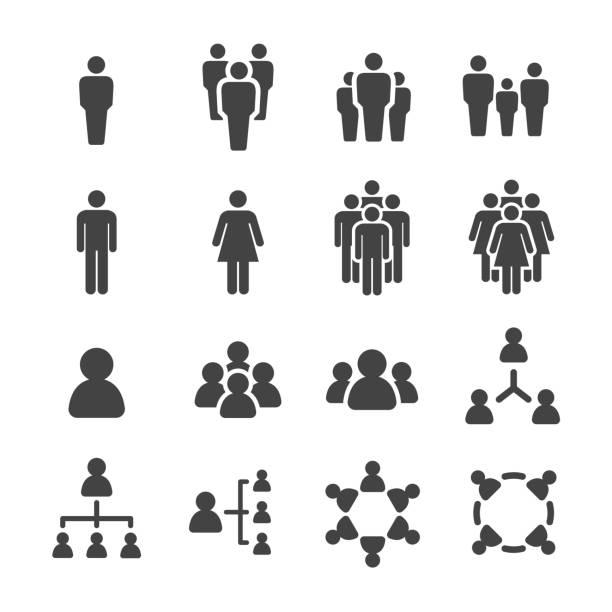
\includegraphics[width=\textwidth]{images/freg-bilde.jpg}
                \end{center}
            \end{column}
        \end{columns}
    \end{frame}


    %%%%%%%%%%%%%%%%%%%%%%%%%%%%%%%%%%%%%%%%%%%%%%%%%%%%%%%%%%%%%%%%%%%%%%%%%%%%%%%%%%%%%%
    % Core Idea
    %%%%%%%%%%%%%%%%%%%%%%%%%%%%%%%%%%%%%%%%%%%%%%%%%%%%%%%%%%%%%%%%%%%%%%%%%%%%%%%%%%%%%%
    \begin{frame}
        \frametitle{Core Idea}
        \begin{itemize}
            \item OpenAPI generates Kotlin classes.
            \item Jackson uses reflection to create objects.
            \item Reflection is slow
            \item Spec contains all info needed to deserialize
            \item Generating the deserializer
        \end{itemize}
    \end{frame}


    %%%%%%%%%%%%%%%%%%%%%%%%%%%%%%%%%%%%%%%%%%%%%%%%%%%%%%%%%%%%%%%%%%%%%%%%%%%%%%%%%%%%%%
    % OpenAPI specification
    %%%%%%%%%%%%%%%%%%%%%%%%%%%%%%%%%%%%%%%%%%%%%%%%%%%%%%%%%%%%%%%%%%%%%%%%%%%%%%%%%%%%%%
    \begin{frame}[fragile]
        \frametitle{OpenAPI Specification}
        \begin{itemize}
            \item Standard to describe RestAPIs
            \begin{itemize}
                \item Http Calls
                \item JSON model for input and output data
            \end{itemize}
            \item Generate model:
            \begin{itemize}
                \item Code for most languages
                \item Model classes
                \item HTTP clients
            \end{itemize}
        \end{itemize}
    \end{frame}


    %%%%%%%%%%%%%%%%%%%%%%%%%%%%%%%%%%%%%%%%%%%%%%%%%%%%%%%%%%%%%%%%%%%%%%%%%%%%%%%%%%%%%%
    % 3 Levels of parsing
    %%%%%%%%%%%%%%%%%%%%%%%%%%%%%%%%%%%%%%%%%%%%%%%%%%%%%%%%%%%%%%%%%%%%%%%%%%%%%%%%%%%%%%
    \begin{frame}
        \frametitle{Jackson: 3 levels of parsing}
        \begin{enumerate}
            \item JsonTokenizer
            \begin{itemize}
                \item Reads JSON as a stream, and divides into tokens
                \item FIELD, VALUE, START\_OBJECT, \ldots
            \end{itemize}
            \item NodeTree
            \begin{itemize}
                \item Reads JSON into a generic tree structure
                \item Primitives, Map<String, JsonNode>, List<JsonNode>
            \end{itemize}
            \item Custom Kotlin / Java Objects (Value)
            \begin{itemize}
                \item MyObj, List<MyObj>, Map<String, MyObj>
                \item Uses reflection to map to Kotlin objects
                \item Reflection is slow
            \end{itemize}
        \end{enumerate}

        \textbf{Number 3 is what we want}
    \end{frame}


    %%%%%%%%%%%%%%%%%%%%%%%%%%%%%%%%%%%%%%%%%%%%%%%%%%%%%%%%%%%%%%%%%%%%%%%%%%%%%%%%%%%%%%
    % How OpenAPI generate classes
    %%%%%%%%%%%%%%%%%%%%%%%%%%%%%%%%%%%%%%%%%%%%%%%%%%%%%%%%%%%%%%%%%%%%%%%%%%%%%%%%%%%%%%
    \definecolor{bg}{rgb}{0.95,0.95,0.95}

    \defverbatim[colored]\runOpenAPIGenerator{
        \begin{zshcode}
    # Generate code
    java -jar openapi-generator-cli.jar generate \
    -g kotlin --template-dir ./openapi-templates \
    -c openapi-generator-config.yaml \
    -o tmp \
    -i src/main/resources/openapi/freg-api-offentlig-med-hjemmel.json \
    --package-name im.kny.jacksonspeedup.offentligmedhjemmel

    # Copy in the code
    srcdir="src/main/kotlin/im/kny/jacksonspeedup/offentligmedhjemmel"
    rm -rf \${srcdir}/models/
    mv tmp/\${srcdir}/models \${srcdir}/
        \end{zshcode}
    }

    \begin{frame}
        \frametitle{How OpenAPI generate classes}
        \begin{itemize}

            \item Include Deserializer
            \href{file:///home/kny/src/personal/jackson-speedup/openapi-templates/data_class.mustache}{data\_class.mustache}

            \item Deserializer
            \href{file:/home/kny/src/personal/jackson-speedup/openapi-templates/jackson_deserializer.mustache}{jackson\_deserializer.mustache}

            \item Value deserializer
            \href{file:///home/kny/src/personal/jackson-speedup/openapi-templates/jackson_deserializer.mustache}{deserialize\_value.mustache}
        \end{itemize}

    \end{frame}




    %%%%%%%%%%%%%%%%%%%%%%%%%%%%%%%%%%%%%%%%%%%%%%%%%%%%%%%%%%%%%%%%%%%%%%%%%%%%%%%%%%%%%%
    % Generate new code
    %%%%%%%%%%%%%%%%%%%%%%%%%%%%%%%%%%%%%%%%%%%%%%%%%%%%%%%%%%%%%%%%%%%%%%%%%%%%%%%%%%%%%%
    \begin{frame}
        \frametitle{Generate Code}

        \runOpenAPIGenerator

    \end{frame}



    %%%%%%%%%%%%%%%%%%%%%%%%%%%%%%%%%%%%%%%%%%%%%%%%%%%%%%%%%%%%%%%%%%%%%%%%%%%%%%%%%%%%%%
    % The End
    %%%%%%%%%%%%%%%%%%%%%%%%%%%%%%%%%%%%%%%%%%%%%%%%%%%%%%%%%%%%%%%%%%%%%%%%%%%%%%%%%%%%%%
    \begin{frame}
        \frametitle{Thank you for your attention}
        If you want to see example code: \url{https://github.com/kny78/jackson-speedup/}

    \end{frame}


\end{document}